


\colorlet{tp}{teal!50!purple}



\AddToShipoutPictureFG{

\ifnum\value{page}=4{
\AtTextLowerLeft{\raisebox{575pt}{

\begin{tikzpicture}

\node at (0,0) [text=white] {X};

%\draw (.6,4.3) circle  (6pt) [xscale=1.4];
%\draw (1,0) circle (6pt);

\node [draw, circle, minimum size=8pt,xscale=2.7, 
draw=teal!40!black] (s1) at (.63,4.24) {};


\node [draw, circle, minimum size=8pt,xscale=2.7, 
draw=teal!40!black] (n1) at (.93,11.29) {};


\node [draw, rectangle, minimum width=40pt, minimum height=13pt, 
anchor = south west, rounded corners,
draw=teal!40!black] (s2) at (4.78,3.2) {};


\node [draw, rectangle, minimum width=40pt, minimum height=13pt, 
anchor = south west, rounded corners,
draw=teal!40!black] (n2) at (9.3,10.78) {};


\node [draw, rectangle, minimum width=40pt, minimum height=13pt, 
anchor = south west, rounded corners,
draw=teal!40!black] (n3) at (13.7,10.78) {};




\node [draw, rectangle, minimum width=40pt, minimum height=13pt, 
anchor = south west, rounded corners,
draw=teal!40!black] (s3) at (18.65,4.53) {};



\node [draw=red!60!black, fill=blue, anchor = south west, rounded corners,
text width=6cm, inner sep=19pt, xshift=-8pt, yshift=-8pt, font={\fontsize{9}{9}\selectfont}] (ltext)
 at (.64, 6.1) {{A PacTk split-window GUI showing index entry matches 
in PDF view and raw text.  PacTk identifies the matching page numbers 
and paragraph codes, and shows how the match appears in raw text 
to help the user check whether the match should be added to the 
index metadata.}
};


\node [draw=red!60!black, fill=white, anchor = south west, rounded corners,
text width=6cm, inner sep=13pt, font={\fontsize{9}{9}\selectfont}] (ltext-outer)
 at (.64, 6.1) {A PacTk split-window GUI showing index entry matches 
in PDF view and raw text.  PacTk identifies the matching page numbers 
and paragraph codes, and shows how the match appears in raw text 
to help the user check whether the match should be added to the 
index metadata.
};


\draw  [->,>=stealth', line width=4pt, draw=tp!50] ([yshift=3pt] s1.east) to 
  [bend right=30, in=180, out=0] ([yshift=-4pt, xshift=-23pt] ltext.south) ;

\draw  [->,>=stealth', line width=4pt, draw=tp!50] ([yshift=3pt] s2.north) to 
  [bend right=10, in=180, out=20] ([yshift=-4pt] ltext.south) ;


\draw  [->,>=stealth', line width=4pt, draw=tp!50] ([yshift=3pt] s3.west) to 
  [bend right, in=120, out=0] ([yshift=-4pt, xshift=33pt] ltext.south) ;



\draw  [->,>=stealth', line width=4pt, draw=tp!50] ([yshift=-3pt, xshift=9pt] n1.south) to 
  [bend right=10, in=180, out=-20]
  ([yshift=4pt, xshift=-43pt] ltext.north) ;


\draw  [->,>=stealth', line width=4pt, draw=tp!50] ([yshift=-3pt] n2.west) to 
  [bend right=10, in=-90, out=0] ([yshift=4pt, xshift=-2pt] ltext.north) ;

\draw  [->,>=stealth', line width=4pt, draw=tp!50] ([yshift=-3pt] n3.west) to 
  [bend right=4] ([yshift=4pt, xshift=79pt] ltext.north) ;


%\draw (ltext) -- (s1);
%



\node [draw, rectangle, minimum width=340pt, minimum height=40pt, 
anchor = south west, rounded corners,
draw=teal!40!black] at (6.8,.76) {};


\node [draw=red!60!black, fill=blue, anchor = south west, rounded corners,
text width=5cm, inner sep=17pt, xshift=-8pt, yshift=-8pt, font={\fontsize{9}{9}\selectfont}] (ltext)
 at (15.4, .8) {{For this workflow, PacTk constructs an index in HTML that can then 
be converted into print-style pages for a physical book and/or merged into a 
composite online meta-index.
}
};


\node [draw=red!60!black, fill=white, anchor = south west, rounded corners,
text width=5cm, inner sep=13pt, font={\fontsize{9}{9}\selectfont}] (ltext-outer)
 at (15.26, .64) {For this workflow, PacTk constructs an index in HTML that can then 
be converted into print-style pages for a physical book and/or merged into a 
composite online meta-index.
};





\node [draw, rectangle, minimum width=149pt, minimum height=50pt, 
anchor = south west, rounded corners,
draw=teal!40!black] at (6.8,3.96) {};


\node [draw=red!60!black, fill=blue, anchor = south west, rounded corners,
text width=4.5cm, inner sep=17pt, xshift=-8pt, yshift=-8pt, font={\fontsize{9}{9}\selectfont}] (ltext)
 at (9.4, 5.2) {{GUI controls let users refine search terms -- especially 
phrases based on index entries --  
by rearranging words and/or selecting the most significant words from a 
longer phrase.
}
};


\node [draw=red!60!black, fill=white, anchor = south west, rounded corners,
text width=4.5cm, inner sep=13pt, font={\fontsize{9}{9}\selectfont}] (ltext-outer)
 at (9.26, 5.14) {GUI controls let users refine search terms -- especially 
phrases based on index entries --   
by rearranging words and/or selecting the most significant words from a 
longer phrase.
};





\end{tikzpicture}


}}


}\fi



\ifnum\value{page}=5{
\AtTextLowerLeft{\raisebox{345pt}{

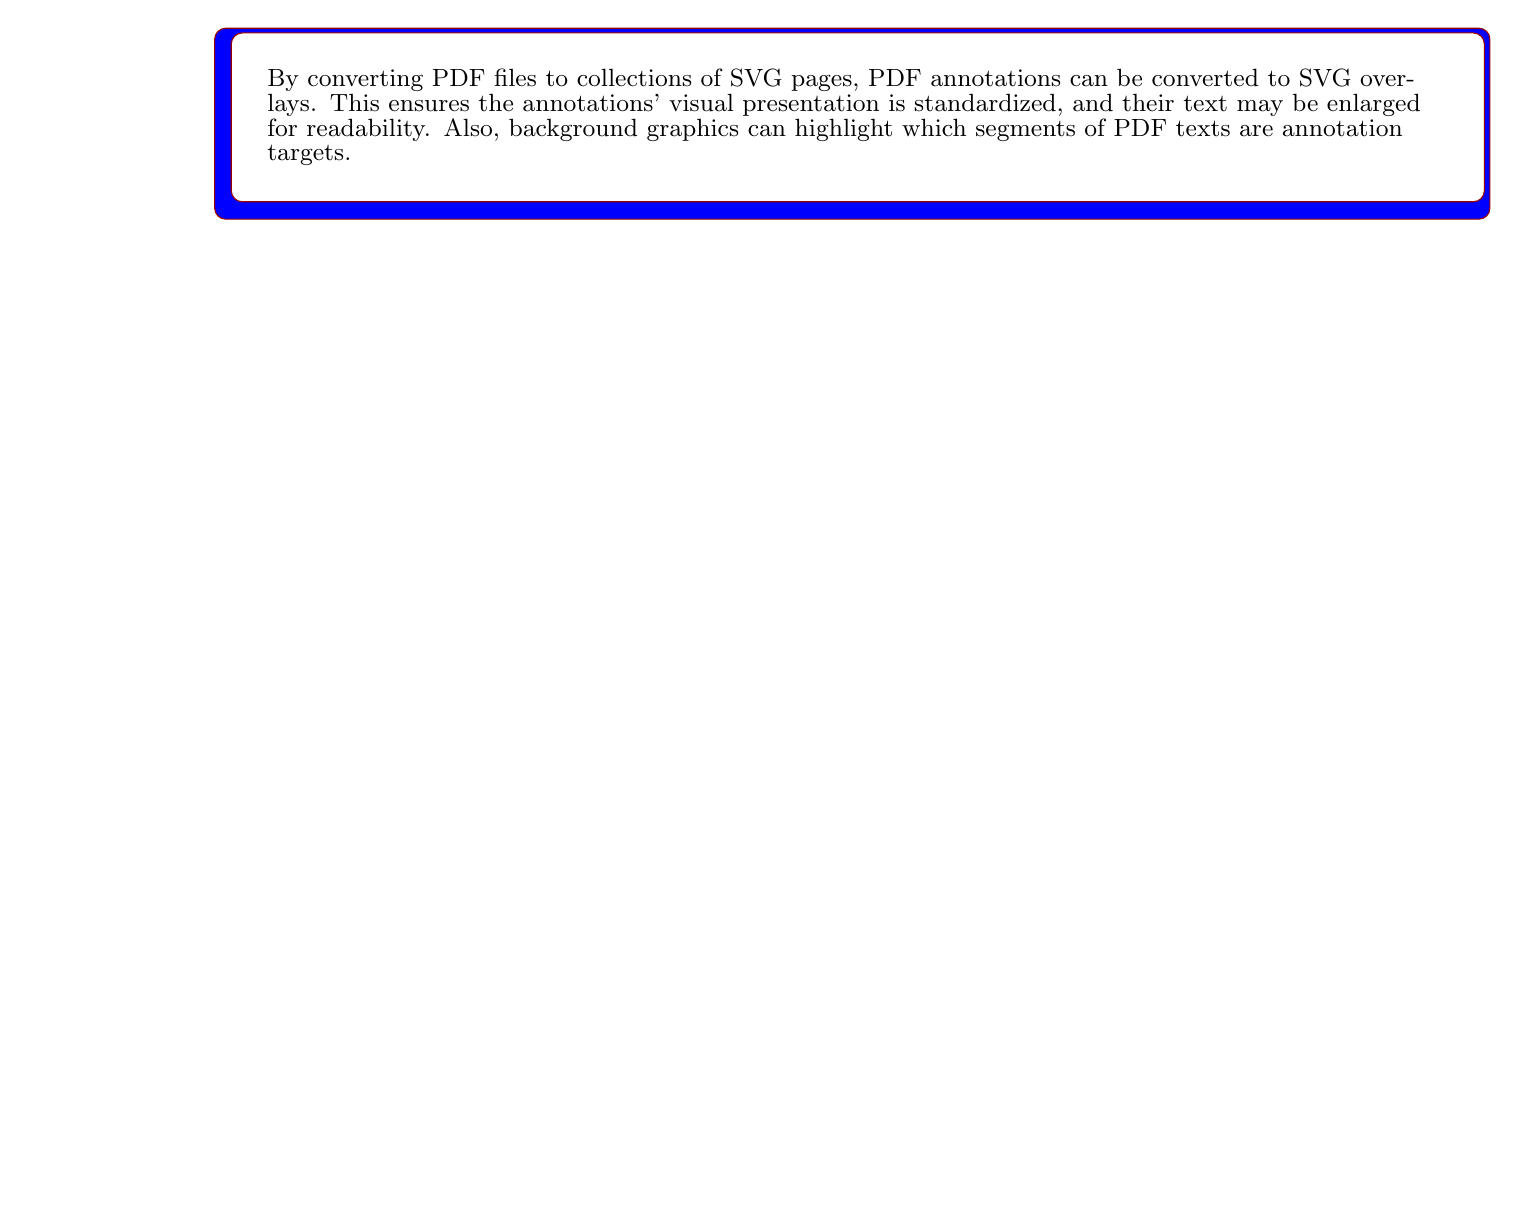
\begin{tikzpicture}

\node at (0,0) [text=white] {X};




\node [draw=red!60!black, fill=blue, anchor = south west, rounded corners,
text width=15cm, inner sep=17pt, xshift=-8pt, yshift=-8pt, font={\fontsize{9}{9}\selectfont}] (ltext)
(s1) at (2.4, 12.4) {{By converting PDF files to collections of SVG pages, PDF annotations 
can be converted to SVG overlays.  This \makebox{ensures} the annotations' visual presentation 
is standardized, and their text may be enlarged for readability.  Also, background 
graphics can highlight which segments of PDF texts are annotation targets.
}
};


\node [draw=red!60!black, fill=white, anchor = south west, rounded corners,
text width=15cm, inner sep=13pt, font={\fontsize{9}{9}\selectfont}] (ltext-outer)
 at (2.33, 12.34) {By converting PDF files to collections of SVG pages, PDF annotations 
can be converted to SVG overlays.  This \makebox{ensures} the annotations' visual presentation 
is standardized, and their text may be enlarged for readability.  Also, background 
graphics can highlight which segments of PDF texts are annotation targets.
};

\end{tikzpicture}
}}

}\fi







\ifnum\value{page}=6{
\AtTextLowerLeft{\raisebox{525pt}{

\begin{tikzpicture}

\node at (0,0) [text=black!7] {X};




\node [draw=red!60!black, fill=blue, anchor = south west, rounded corners,
text width=15cm, inner sep=17pt, xshift=-8pt, yshift=-8pt, font={\fontsize{9}{9}\selectfont}] (ltext)
 at (2.4, 12.2) {{Converting PDF files to SVG pages also allows each page to 
have its own web address.  This enables publishers to organize pages 
into an online concordance indexed by topic or by annotated content.
}
};


\node [draw=red!60!black, fill=white, anchor = south west, rounded corners,
text width=15cm, inner sep=13pt, font={\fontsize{9}{9}\selectfont}] (ltext-outer)
 at (2.33, 12.14) {Converting PDF files to SVG pages also allows each page to 
have its own web address.  This enables publishers to organize pages 
into an online concordance indexed by topic or by annotated content.
};





\node [draw=red!60!black, fill=blue, anchor = south west, rounded corners,
text width=18cm, inner sep=17pt, xshift=-8pt, yshift=-8pt, font={\fontsize{9}{9}\selectfont}] (ltext)
 at (.4, 4.2) {{In this case, a concordance was compiled by grouping pages 
into categories based on annotations.  The concordance was then 
published online as a master index, with links for each page presented 
alongside a checkbox-based table showing the category 
distribution per page.
}
};


\node [draw=red!60!black, fill=white, anchor = south west, rounded corners,
text width=18cm, inner sep=13pt, font={\fontsize{9}{9}\selectfont}] (ltext-inner)
 at (.33, 4.1) {In this case, a concordance was compiled by grouping pages 
into categories based on annotations.  The concordance was then 
published online as a master index, with links for each page presented 
alongside a checkbox-based table showing the category 
distribution per page.
};


\node [draw, rectangle, minimum width=165pt, minimum height=28pt, 
anchor = south west, rounded corners,
draw=teal!40!black] (s1) at (.7,.33) {};


\draw  [->,>=stealth', line width=4pt, draw=tp!50] ([yshift=13pt] s1.south east) to 
  [bend right=40, in=-90, out=-20] ([yshift=4pt, xshift=243pt] ltext.south) ;




\node [draw=red!60, fill=white, anchor = south west, rounded corners,
text width=4cm, inner sep=4pt, font={\fontsize{9}{9}\selectfont}] (stext)
 at (11.33, 1.6) {HTML columns were derived from a controlled vocabulary 
adopted for annotation text.
};

\draw  [--,>=stealth', line width=4pt, draw=tp!50] ([yshift=3pt, xshift=5pt] s1.south east) to 
   ([yshift=18pt, xshift=220] s1.south east) ;


\draw  [->,>=stealth', line width=4pt, draw=tp!50] ([yshift=18pt, xshift=218] s1.south east) to 
   ([yshift=3, xshift=20] stext.south) ;



\end{tikzpicture}
}}

}\fi








\ifnum\value{page}=8{
\AtTextLowerLeft{\raisebox{515pt}{

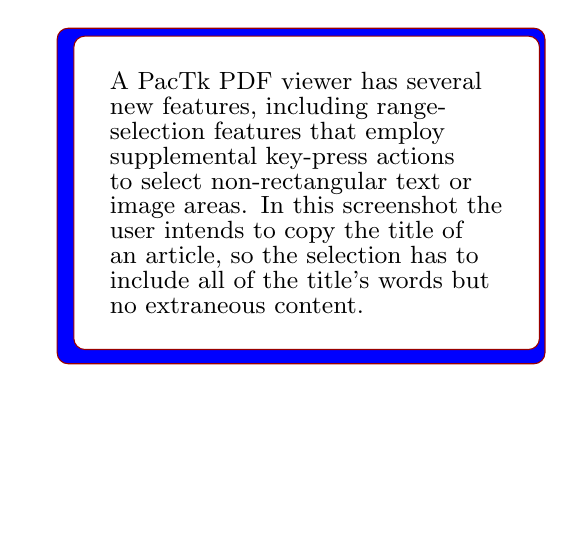
\begin{tikzpicture}

\node at (0,0) [text=white] {X};




\node [draw=red!60!black, fill=blue, anchor = south west, rounded corners,
text width=5cm, inner sep=17pt, xshift=-8pt, yshift=-8pt, font={\fontsize{9}{9}\selectfont}] (ltext)
(s1) at (.4, 1.9) {{A PacTk PDF viewer has several new features, including range-selection 
features that employ supplemental key-press actions to select non-rectangular 
text or image areas.  In this screenshot the user intends to copy the title 
of an article, so the selection has to include all of the title's words 
but no extraneous content.
}
};


\node [draw=red!60!black, fill=white, anchor = south west, rounded corners,
text width=5cm, inner sep=13pt, font={\fontsize{9}{9}\selectfont}] (ltext-outer)
 at (.33, 1.8) {A PacTk PDF viewer has several new features, including range-selection 
features that employ supplemental key-press actions to select non-rectangular 
text or image areas.  In this screenshot the user intends to copy the title 
of an article, so the selection has to include all of the title's words 
but no extraneous content.
};

\end{tikzpicture}
}}

}\fi









\ifnum\value{page}=3{
\AtTextLowerLeft{\raisebox{415pt}{

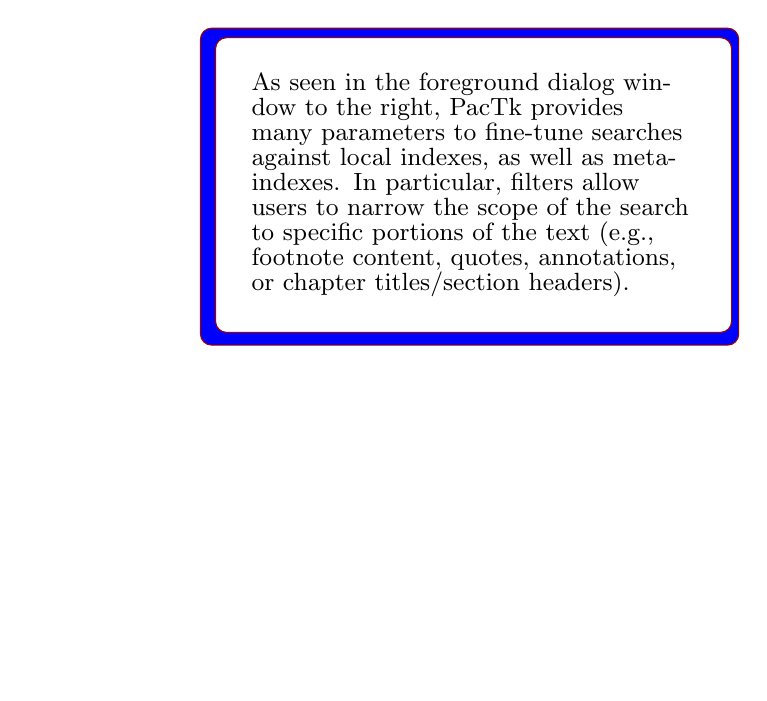
\begin{tikzpicture}

\node at (0,0) [text=white] {X};




\node [draw=red!60!black, fill=blue, anchor = south west, rounded corners,
text width=5.64cm, inner sep=17pt, xshift=-8pt, yshift=-8pt, font={\fontsize{9}{9}\selectfont}] (ltext)
(s1) at (2.22, 4.2) {{As seen in the foreground dialog window to the right, PacTk provides many 
parameters to fine-tune searches against local indexes, as well as meta-indexes.  
In particular, filters allow users to narrow the scope of the search 
to specific portions of the text (e.g., footnote content, quotes, 
annotations, or chapter titles/section headers).
}
};


\node [draw=red!60!black, fill=white, anchor = south west, rounded corners,
text width=5.64cm, inner sep=13pt, font={\fontsize{9}{9}\selectfont}] (ltext-outer)
 at (2.13, 4.08) {
As seen in the foreground dialog window to the right, PacTk provides many 
parameters to fine-tune searches against local indexes, as well as meta-indexes.  
In particular, filters allow users to narrow the scope of the search 
to specific portions of the text (e.g., footnote content, quotes, 
annotations, or chapter titles/section headers).
};

\end{tikzpicture}
}}

}\fi







\ifnum\value{page}=2{
\AtTextLowerLeft{\raisebox{415pt}{

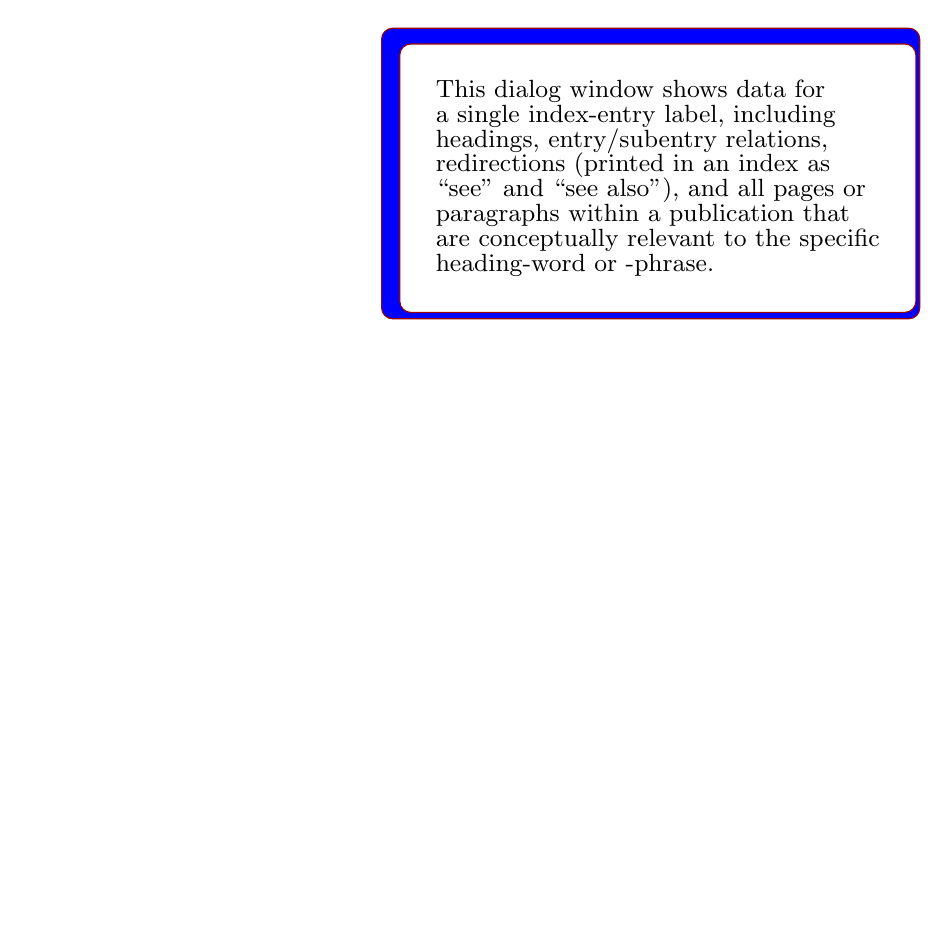
\begin{tikzpicture}

\node at (0,0) [text=white] {X};


\node [draw=red!60!black, fill=blue, anchor = south west, rounded corners,
text width=5.64cm, inner sep=17pt, xshift=-8pt, yshift=-8pt, font={\fontsize{9}{9}\selectfont}] (ltext)
(s1) at (4.52, 7.7) {{
This dialog window shows data for a single index-entry label, including entry/subentry 
relations, redirections (printed in an index as ``see'' and ``see also''), 
headings, and all pages or paragraphs within a publication that 
are conceptually relevant to the specific heading-word or -phrase.
}
};


\node [draw=red!60!black, fill=white, anchor = south west, rounded corners,
text width=5.64cm, inner sep=13pt, font={\fontsize{9}{9}\selectfont}] (ltext-outer)
 at (4.47, 7.5) {
This dialog window shows data for a single index-entry label, including \makebox{headings}, 
entry/subentry 
relations, redirections (printed in an index as ``see'' and ``see also''), 
and all pages or paragraphs within a publication that 
are conceptually relevant to the specific heading-word or -phrase.
};

\end{tikzpicture}
}}

}\fi




\ifnum\value{page}=10{
\AtTextLowerLeft{\raisebox{355pt}{

\begin{tikzpicture}

\node at (0,0) [text=black] {X};

\begin{scope}[transform canvas={scale=0.6, shift={(24.6,24.5)}},overlay]

\draw [rotate=20.9245, fill=white] (-1.5pt, 0pt) -- ++(up:5pt) -- ++(-5pt, -2pt) -- ++(6.5pt, 17pt)
                      -- ++(6.5pt, -17pt) -- ++(-5pt, 2pt) -- ++(down:5pt) -- cycle;

\end{scope}

\end{tikzpicture}
}}

}\fi




\ifnum\value{page}=7{
\AtTextLowerLeft{\raisebox{155pt}{

\begin{tikzpicture}

\node at (0,0) [text=black] {X};

\begin{scope}[transform canvas={scale=0.6, shift={(21.6,18.5)}},overlay]

\draw [rotate=20.9245, fill=white] (-1.5pt, 0pt) -- ++(up:5pt) -- ++(-5pt, -2pt) -- ++(6.5pt, 17pt)
                      -- ++(6.5pt, -17pt) -- ++(-5pt, 2pt) -- ++(down:5pt) -- cycle;

\end{scope}

\end{tikzpicture}
}}

}\fi




\ifnum\value{page}=9{
\AtTextLowerLeft{\raisebox{575pt}{

\begin{tikzpicture}

\node at (0,0) [text=white] {X};


\node [draw=red!60!black, fill=blue, anchor = north west, rounded corners,
text width=14.64cm, inner sep=17pt, xshift=-8pt, yshift=-8pt, font={\fontsize{9}{9}\selectfont}] (ltext)
(s1) at (3.52, 11.64) {{
PacTk enables fine-grained metadata to be embedded in documents, representing 
PDF page coordinates for sentence and paragraph start/end points, as well as 
locations for keywords, proper names (and other Named Entities), 
figure illustrations, and other publication landmarks.   
}
};


\node [draw=red!60!black, fill=white, anchor = north west, rounded corners,
text width=14.64cm, inner sep=13pt, font={\fontsize{9}{9}\selectfont}] (ltext-inner)
 at (3.43, 11.2) {
PacTk enables fine-grained metadata to be embedded in documents, representing 
PDF page coordinates for sentence and paragraph start/end points, as well as 
locations for keywords, proper names (and other Named Entities), 
figure illustrations, and other publication landmarks.
};





\node [draw=red!60!black, fill=blue, anchor = north west, rounded corners,
text width=7.64cm, inner sep=17pt, xshift=-8pt, yshift=-8pt, font={\fontsize{9}{9}\selectfont}] 
(stext) at (.3, 2.64) {{
With a conformant PDF viewer, users can examine PacTk metadata directly, which 
can be useful for programmers intending to develop text-mining algorithms.  
}
};


\node [draw=red!60!black, fill=white, anchor = north west, rounded corners,
text width=7.64cm, inner sep=13pt, font={\fontsize{9}{9}\selectfont}] (stext-inner)
 at (.25, 2.2) {
With a conformant PDF viewer, users can examine PacTk metadata directly, which 
can be useful for programmers intending to develop text-mining algorithms.  
};


\draw  [->,>=stealth', line width=4pt, draw=tp!50] ([yshift=48pt, xshift=148] stext.east) to 
  [bend left=20]  ([yshift=-22, xshift=2] stext.east) ;


\draw  [->,>=stealth', line width=4pt, draw=tp!50] ([yshift=28pt, xshift=-18] stext.north) to 
  [bend left=20]  ([yshift=2, xshift=2] stext.north) ;


\draw  [->,>=stealth', line width=4pt, draw=tp!30!magenta] ([yshift=89pt, xshift=179] stext.north) to 
  [bend left=20]  ([yshift=128pt, xshift=274] stext.north) ;


\end{tikzpicture}
}}

}\fi



}

